\documentclass[12pt,letterpaper]{article}

\usepackage{amsmath,amssymb,amsthm,mathrsfs,mathtools,accents}
\usepackage{geometry,xcolor,color,soul}
\usepackage{tikz}
\usepackage[noabbrev, capitalize]{cleveref}

\usepackage{arydshln}

\geometry{
letterpaper,
left=20mm,
right=20mm,
top=20mm,
bottom=20mm
}

\begin{document}
\begin{center}
   \textbf{Example graphs}
\end{center}

\begin{center}
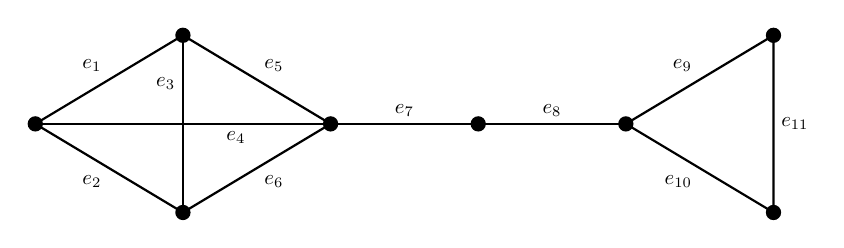
\begin{tikzpicture}[thick, main/.style={draw, circle, fill=black}, scale=1.5, every node/.style={scale=0.5}]

	\node[main] (1) at (-2.5, 0) {};
	\node[main] (2) at (-1.25, 0.75) {};
	\node[main] (3) at (-1.25, -0.75) {};
	\node[main] (4) at (0,0) {};
	
	\node[main] (5) at (1.25,0) {};
	\node[main] (6) at (2.5,0) {};
	\node[main] (7) at (3.75, 0.75) {};
	\node[main] (8) at (3.75, -0.75) {};
	
	\draw (1) -- (2) node [midway, above left, scale=1.5] {$e_1$};
	\draw (1) -- (3) node [midway, below left, scale=1.5] {$e_2$};
	\draw (2) -- (3) node [near start, left, scale=1.5] {$e_3$};
	\draw (1) -- (4) node [near end, below left, scale=1.5] {$e_4$};
	\draw (2) -- (4) node [midway, above right, scale=1.5] {$e_5$};
	\draw (3) -- (4) node [midway, below right, scale=1.5] {$e_6$};
	\draw (4) -- (5) node [midway, above, scale=1.5] {$e_7$};
	\draw (5) -- (6) node [midway, above, scale=1.5] {$e_8$};
	\draw (6) -- (7) node [midway, above left, scale=1.5] {$e_9$};
	\draw (6) -- (8) node [midway, below left, scale=1.5] {$e_{10}$};
	\draw (7) -- (8) node [midway, right, scale=1.5] {$e_{11}$};
	
\end{tikzpicture}
\end{center}

\begin{verbatim}
R = QQ[e_1..e_11]
I = ideal(e_2*e_5-e_1*e_6,e_3*e_4-e_1*e_6,e_3*e_7^2*e_9*e_10-e_5*e_6*e_8^2*e_11,
e_2*e_7^2*e_9*e_10-e_4*e_6*e_8^2*e_11,e_1*e_7^2*e_9*e_10-e_4*e_5*e_8^2*e_11)	
\end{verbatim}

\begin{center}
\begin{tabular}{c|c|c|c}
	{\bf trial} & {\bf shipping version} & {\bf oneStep changes} & {\bf oneStep \& tgb changes}
	\\ \hline\hline
	1 & 475s & 415s &  \\ \hline 
	2 & 471s & 414s &  \\ \hline 
	3 & 474s & 411s &  \\ \hline 
	4 & 471s & 411s &  \\ \hline 
	5 & 474s & 411s &  \\ \hline
	\hline 
	avg. & 473s & 412s &  \\ \hdashline 
	difference & --- &  61s quicker
\end{tabular}	
\end{center}

\noindent
\hrulefill

Removing one edge:

\begin{center}
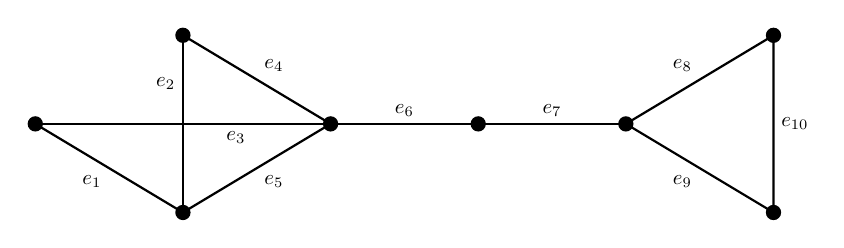
\begin{tikzpicture}[thick, main/.style={draw, circle, fill=black}, scale=1.5, every node/.style={scale=0.5}]

	\node[main] (1) at (-2.5, 0) {};
	\node[main] (2) at (-1.25, 0.75) {};
	\node[main] (3) at (-1.25, -0.75) {};
	\node[main] (4) at (0,0) {};
	
	\node[main] (5) at (1.25,0) {};
	\node[main] (6) at (2.5,0) {};
	\node[main] (7) at (3.75, 0.75) {};
	\node[main] (8) at (3.75, -0.75) {};
	
	\draw (1) -- (3) node [midway, below left, scale=1.5] {$e_1$};
	\draw (2) -- (3) node [near start, left, scale=1.5] {$e_2$};
	\draw (1) -- (4) node [near end, below left, scale=1.5] {$e_3$};
	\draw (2) -- (4) node [midway, above right, scale=1.5] {$e_4$};
	\draw (3) -- (4) node [midway, below right, scale=1.5] {$e_5$};
	\draw (4) -- (5) node [midway, above, scale=1.5] {$e_6$};
	\draw (5) -- (6) node [midway, above, scale=1.5] {$e_7$};
	\draw (6) -- (7) node [midway, above left, scale=1.5] {$e_8$};
	\draw (6) -- (8) node [midway, below left, scale=1.5] {$e_9$};
	\draw (7) -- (8) node [midway, right, scale=1.5] {$e_{10}$};
	
\end{tikzpicture}
\end{center}

\begin{verbatim}
R = QQ[e_1..e_10]
I = ideal(e_2*e_3-e_1*e_4,e_2*e_6^2*e_8*e_9-e_4*e_5*e_7^2*e_10,
e_1*e_6^2*e_8*e_9-e_3*e_5*e_7^2*e_10)	
\end{verbatim}

\begin{center}
\begin{tabular}{c|c|c|c}
	{\bf trial} & {\bf shipping version} & {\bf oneStep changes} & {\bf oneStep \& tgb changes}
	\\ \hline\hline
	1 & 14.7s & 13.2s &  \\ \hline 
	2 & 14.8s & 13.2s &  \\ \hline 
	3 & 14.7s & 13.1s &  \\ \hline 
	4 & 14.9s & 13.1s &  \\ \hline 
	5 & 14.9s & 13.3s &  \\ \hline 
	\hline 
	avg. & 14.8s & 13.18s &  \\ \hdashline
	difference & --- & 1.62s quicker
\end{tabular}	
\end{center}


	
\end{document}


















